\documentclass[en]{../../../eplsummary}

\usetikzlibrary{calc, trees, positioning, arrows, shapes, shapes.multipart, shadows, matrix, decorations.pathreplacing, decorations.pathmorphing}
\usetikzlibrary{arrows,shapes,snakes,automata,backgrounds,petri}

\hypertitle{cloud-INGI2145}{7}{INGI}{2145}
{Houtain Nicolas, Thibault Gérondal}
{Canini Marco}

\section{Cloud computing}

\subsection{Introduction}

\begin{center}
    \textit{Cloud computing is a model for enabling convenient, 
        on-­demand network access to a shared pool of configurable 
        computing resources (e.g., networks, servers, storage, 
        applications, and services) that can be rapidly provisioned 
        and released with minimal management effort or 
    service provider interaction.}
\end{center}

\begin{tabular}{cm{10cm}}
    \textbf{Cloud commandments} &
    \begin{enumerate}
        \item Partition everything
        \item Use asynchony everywhere
        \item Automate everything
        \item Remember that everything fails
        \item Embrace inconsistency
    \end{enumerate}
\end{tabular}

\begin{tabular}{cm{10cm}}
    \textbf{Cloud benefit} &
    \begin{itemize}
        \item Elastic, just-­in-­time infrastructure
        \item More efficient resource utilization
        \item Pay for what you use
        \item Potential to reduce processing time (parallelization)
        \item Leverage multiple data centers (high availability)
    \end{itemize}
\end{tabular}


\subsubsection{Hardware scalability}

Cloud need for \textbf{scalability} because modern application require
huge amounts of processing and data. Cluster (\textit{room-sized}) and datacenter 
(\textit{building-sized}) can provide the resources needed.
They are composed of \textbf{rack} which is a aggregation of storage devices, many
nodes and switch to connect nodes together. Unfortunately, they are not perfect.
\begin{enumerate}
    \item Difficult to dimension because they must be provisioning for the peak load
    \item Expensive in hardware invest, expertise (ex: special software) and maintenance
    \item Difficult to scale because adding new machines is not easy
\end{enumerate}


\subsubsection{Model}
Cloud computing is a business models where everything is a service:
\begin{itemize}
    \item \textbf{SaaS}: Software as a service
    \item \textbf{PaaS}: Platform as a service
    \item \textbf{IaaS}: Infrastructure as a service
\end{itemize}

\subsubsection{Types}
There also have three types of cloud : 
\begin{itemize}
    \item \textbf{Public}: commercial commercial service open to almost anyone.
    \item \textbf{Community}: shared by several similar organization
    \item \textbf{Private}: shared within a organization
\end{itemize}
In this course we focus on public cloud.

\subsubsection{Applications}

Typically, applications that involve large amounts of computation, storage,
bandwidth Especially when lots of resources are needed quickly or load varies
rapidly.

\begin{itemize}
    \item \textbf{Web app}: Near the edge of the application focus is on vast 
        numbers of clients and rapid response
    \item \textbf{Processing pipelines}: Inside we find data-­intensive services that 
        operate in a pipelined manner, asynchronously
    \item \textbf{Batch processing}: Deep inside the application we see a world of 
        virtual computer clusters that are scheduled to 
        share resources and on which applications like 
        MapReduce (Hadoop) are very popular
\end{itemize}


\subsubsection{Virtualization}
IS used to simulate multiple physical machine for the consumer with different
capabilities. It's powerful for security and isolation because VM cannot influence
other. In the other hand, performance is hard to predict because other VM run on
the same physical machine.

\subsubsection{Challenge}
\begin{tabular}{m{0.5\linewidth}m{0.5\linewidth}}
    \begin{itemize}
        \item Availability
        \item Data lock-in (moving data)
        \item Data confidentiality and auditability 
        \item Data transfer bottlenecks
        \item Performance unpredictability for VM
    \end{itemize}
    &
    \begin{itemize}
        \item Scalable storage
        \item Bugs in large distributed systems
        \item Scaling quickly
        \item Reputation fate sharing
        \item Software licensing
    \end{itemize}
\end{tabular}

\section{Summary of Eventually Consistent}

Data inconsistency in large-scale reliable distributed systems has to be tolerated for two reasons: improving read and write performance under highly concurrent conditions; and handling partition cases where a majority model would render part of the system unavailable even though the nodes are up and running.

Whether or not inconsistencies are acceptable depends on the client application. In all cases the developer needs to be aware that consistency guarantees are provided by the storage systems and need to be taken into account when developing applications.

\begin{description}
\item[Strong consistency] After the update completes, any subsequent access (by A, B, or C) will return the updated value.

\item[Weak consistency] The system does not guarantee that subsequent accesses will return the updated value. A number of conditions need to be met before the value will be returned. The period between the update and the moment when it is guaranteed that any observer will always see the updated value is dubbed the inconsistency window.

\item[Eventual consistency] This is a specific form of weak consistency; the storage system guarantees that if no new updates are made to the object, eventually all accesses will return the last updated value. If no failures occur, the maximum size of the inconsistency window can be determined based on factors such as communication delays, the load on the system, and the number of replicas involved in the replication scheme. The most popular system that implements eventual consistency is DNS (Domain Name System). Updates to a name are distributed according to a configured pattern and in combination with time-controlled caches; eventually, all clients will see the update.

\item[The eventual consistency has a number of variations that are important to consider:]

\item[Causal consistency] If process A has communicated to process B that it has updated a data item, a subsequent access by process B will return the updated value, and a write is guaranteed to supersede the earlier write. Access by process C that has no causal relationship to process A is subject to the normal eventual consistency rules.

\item[Read-your-writes consistency] This is an important model where process A, after it has updated a data item, always accesses the updated value and will never see an older value. This is a special case of the causal consistency model.

\item[Session consistency] This is a practical version of the previous model, where a process accesses the storage system in the context of a session. As long as the session exists, the system guarantees read-your-writes consistency. If the session terminates because of a certain failure scenario, a new session needs to be created and the guarantees do not overlap the sessions.

\item[Monotonic read consistency] If a process has seen a particular value for the object, any subsequent accesses will never return any previous values.

\item[Monotonic write consistency] In this case the system guarantees to serialize the writes by the same process. Systems that do not guarantee this level of consistency are notoriously hard to program.

\end{description}

A number of these properties can be combined. For example, one can get monotonic reads combined with session-level consistency. From a practical point of view these two properties (monotonic reads and read-your-writes) are most desirable in an eventual consistency system, but not always required. These two properties make it simpler for developers to build applications, while allowing the storage system to relax consistency and provide high availability.


\section{Design for scale}

A system is scalable if it can easily adapt to 
increased (or reduced) demand.

\subsection{Parallelism programming}

\subsubsection{Vocabulary}
\begin{description}
    \item[Parallelism]: refers to techniques to make programs faster by
        performing several computations in parallel.

    \item[Concurrency]: is the composition of independently executing
        computations.
\end{description}

\subsubsection{Parallelization}
\begin{itemize}
    \item \textbf{Amdahl's law}:

        \begin{tabular}{m{0.5\linewidth}m{0.5\linewidth}}
            $$\quad S = \frac{1}{\alpha +
            \frac{1-\alpha}{N}}$$ where $\alpha$ is the sequential part and $N$ the
            number of cores.
            &
            \includegraphics[width=6cm]{img/amdahl.png}
        \end{tabular}

        The coarse-grain (opposited to fine-grain) parallelism is more efficient
        because he limits the communication and coordination overheads by allow
        bigger task.
    \item \textbf{Dependencies}: Some task need to be after other which limits the degree of 
        parallelism. $\rightarrow$ Scheduling problem
\end{itemize}

\subsubsection{Architecture}
\begin{itemize}
    \item Symmetric multiprocessing (SMP): all processors share same memory.

        \begin{tabular}{m{0.7\linewidth}m{0.3\linewidth}}
            \begin{itemize} 
                \item[+] Simplicity and easy to load balance 
                \item[-] Scalability limited and expensive
            \end{itemize}
            &
            \begin{tiny}
                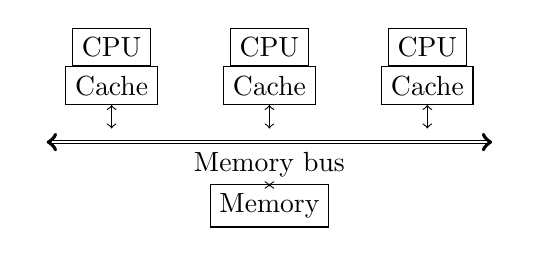
\begin{tikzpicture}
                    \node[draw, rectangle] (1) {CPU};
                    \node[draw, rectangle] (2) [right=of 1] {CPU};
                    \node[draw, rectangle] (3) [right=of 2] {CPU};

                    \node[draw, rectangle] (11) [below=0cm of 1] {Cache};
                    \node[draw, rectangle] (21) [below=0cm of 2] {Cache};
                    \node[draw, rectangle] (31) [below=0cm of 3] {Cache};

                    \node (12) [below=0.3cm of 11] {};
                    \node (22) [below=0.3cm of 21] {};
                    \node (32) [below=0.3cm of 31] {};

                    \node (tmp) [below left= -0.2cm and 0.7cm of 12] {};
                    \node (tmp2) [below right=-0.2cm and 0.7cm of 32] {};

                    \draw (tmp) edge[double, <->] node[below](p) {Memory bus} (tmp2);
                    \draw (12) edge[<->] (11);
                    \draw (22) edge[<->] (21);
                    \draw (32) edge[<->] (31);

                    \node[draw, rectangle] (mem) [below=1.0cm of 21] {Memory};
                    \draw (mem) edge[<->] (p);
                \end{tikzpicture}
            \end{tiny}
        \end{tabular}

    \item Non Uniform memory architecture (NUMA)

        \begin{tabular}{m{0.7\linewidth}m{0.3\linewidth}}
            \begin{itemize} 
                \item[+] Better scalability and faster memory
                \item[-] Complicates programming and scalability limited
            \end{itemize}
            &
            \begin{tiny}
                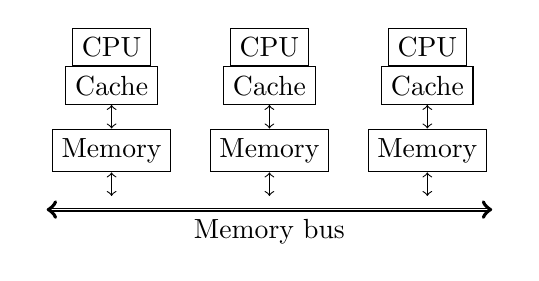
\begin{tikzpicture}
                    \node[draw, rectangle] (1) {CPU};
                    \node[draw, rectangle] (2) [right=of 1] {CPU};
                    \node[draw, rectangle] (3) [right=of 2] {CPU};

                    \node[draw, rectangle] (11) [below=0cm of 1] {Cache};
                    \node[draw, rectangle] (21) [below=0cm of 2] {Cache};
                    \node[draw, rectangle] (31) [below=0cm of 3] {Cache};

                    \node[draw, rectangle] (12) [below=0.3cm of 11] {Memory};
                    \node[draw, rectangle] (22) [below=0.3cm of 21] {Memory};
                    \node[draw, rectangle] (32) [below=0.3cm of 31] {Memory};

                    \node (13) [below=0.3cm of 12] {};
                    \node (23) [below=0.3cm of 22] {};
                    \node (33) [below=0.3cm of 32] {};

                    \node (tmp) [below left= -0.2cm and 0.7cm of 13] {};
                    \node (tmp2) [below right=-0.2cm and 0.7cm of 33] {};

                    \draw (tmp) edge[double, <->] node[below](p) {Memory bus} (tmp2);
                    \draw (12) edge[<->] (11);
                    \draw (22) edge[<->] (21);
                    \draw (32) edge[<->] (31);

                    \draw (12) edge[<->] (13);
                    \draw (22) edge[<->] (23);
                    \draw (32) edge[<->] (33);
                \end{tikzpicture}
            \end{tiny}
        \end{tabular}

    \item Shared Nothing

        \begin{tabular}{m{0.7\linewidth}m{0.3\linewidth}}
            \begin{itemize} 
                \item[+] Nice scalability
                \item[-] Requires different programming model
            \end{itemize}
            &

            \begin{tiny}
                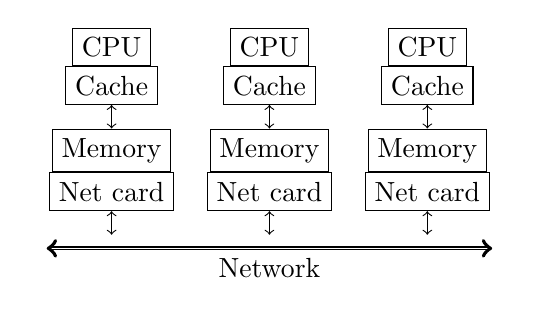
\begin{tikzpicture}
                    \node[draw, rectangle] (1) {CPU};
                    \node[draw, rectangle] (2) [right=of 1] {CPU};
                    \node[draw, rectangle] (3) [right=of 2] {CPU};

                    \node[draw, rectangle] (11) [below=0cm of 1] {Cache};
                    \node[draw, rectangle] (21) [below=0cm of 2] {Cache};
                    \node[draw, rectangle] (31) [below=0cm of 3] {Cache};

                    \node[draw, rectangle] (12) [below=0.3cm of 11] {Memory};
                    \node[draw, rectangle] (22) [below=0.3cm of 21] {Memory};
                    \node[draw, rectangle] (32) [below=0.3cm of 31] {Memory};

                    \node[draw, rectangle] (14) [below=0cm of 12] {Net card};
                    \node[draw, rectangle] (24) [below=0cm of 22] {Net card};
                    \node[draw, rectangle] (34) [below=0cm of 32] {Net card};

                    \node (13) [below=0.3cm of 14] {};
                    \node (23) [below=0.3cm of 24] {};
                    \node (33) [below=0.3cm of 34] {};

                    \node (tmp) [below left= -0.2cm and 0.7cm of 13] {};
                    \node (tmp2) [below right=-0.2cm and 0.7cm of 33] {};

                    \draw (tmp) edge[double, <->] node[below](p) {Network} (tmp2);
                    \draw (12) edge[<->] (11);
                    \draw (22) edge[<->] (21);
                    \draw (32) edge[<->] (31);

                    \draw (13) edge[<->] (14);
                    \draw (23) edge[<->] (24);
                    \draw (33) edge[<->] (34);
                \end{tikzpicture}
            \end{tiny}
        \end{tabular}

\end{itemize}


\subsection{Distributed programming}

\subsubsection{Vocabulary}
\begin{description}
    \item[Faults]: Some component is not working correctly
    \item[Failure]: System as a whole is not working correctly
\end{description}

\subsubsection{Wide-area network}
The transfert speed for some data are defined by some attributs:
\begin{enumerate}
    \item Propagation delay
    \item Bottlenecks capacity on the path
    \item Queueing delay, loss, reordering, congestion, rtt 
        (take in account by TCP)
\end{enumerate}

$\rightarrow$ wide-area networks complicates the communication and faults are
more common

\subsubsection{Faults}

Fault are a common event in distributed system and some faults
are correlated.

\begin{itemize}
    \item \textbf{Crash faults}: node simply stop
    \item \textbf{Rational behavior}: owner manipulates node to increase profit
        (ex: lies on the routes to have traffic through it's own AS)
    \item \textbf{Byzantine faults}: faulty node could do anything (ex: stop, send spam,
        attack other, tell lies,...)
\end{itemize}

To prevent fault, we can \textit{prevent} them by using verification,
\textit{detect} them or \textit{mask} them by using replicas. The problem of
using \textbf{replicas} is to be able to maintain consistency between them!

\subsubsection{Consistency}

\begin{itemize}
    \item \textbf{Strong consistency}: After update completes, all subsequent
        accesses will return the updated value

    \item \textbf{Weak consistency}: After update completes, accesses do not
        necessarily return the updated value;; some condition must be satisfied
        first (such as update needs to reach all the replicas)

    \item \textbf{Eventual consistency}: Specific form of weak consistency: If no
        more updates are made to an object, then eventually all reads will return
        the latest value

    \item \textbf{Causal consistency}: If client A has communicated to client B that it
        has updated a data item, a subsequent access by B will return the updated
        value, and a write is guaranteed to supersede the earlier write. Client C
        that has no causal relationship to client A is subject to the normal
        eventual consistency rules

    \item \textbf{Read-your-writes consistency}: Client A, after it has updated a data
        item, always accesses the updated value and will never see an older
        value.

    \item \textbf{Session consistency}: Like previous case but in the context of a
        session, for as long as the sessions remains alive.

    \item \textbf{Monotonic read consistency}: If client A has has seen a particular value
        for the object, any subsequent accesses will never return any previous
        values

    \item \textbf{Monotonic write consistency}: In this case the system guarantees to
        serialize the writes by the same process
\end{itemize}

We can combine them, and monotonic reads + read-your-write are most desirable
than eventual consistency.

\paragraph{Storage system consistency: example}

We have N nodes that can store data.
To write a value: Pick W replicas and write the value to each, using a fresh timestamp
To read a value:
\begin{itemize}
\item Pick R replicas and read the value from each
\item Return the value with the highest timestamp
\item If any replicas had a lower timestamp, send them the newer value
\end{itemize}

Strong consistency :
\begin{description}
\item[Majority quorum] Always write to and read from a majority of nodes. At least one node knows the most recent value.  tolerate up to ⌈N/2⌉ - 1 crashes. But have to read/write ⌊N/2⌋ + 1 values.
\item[Read/write quorums] Read R nodes, write W nodes, s.t. R + W > N. Adjust performance of reads/writes. But availability can suffer.

\begin{tabular}{m{5cm}m{12cm}}
    \includegraphics[width=3cm]{img/replicas} &
    \includegraphics[width=7cm]{img/replicas2}
    \begin{itemize}
        \item[$\rightarrow$] Strong consistency
    \end{itemize} \\
\end{tabular}
\item[Consensus solutions] Paxos (for crash faults), PBFT (for Byzantine faults). Idea : Correct replicas ``outvote'' faulty ones.
\end{description}
 
The cap theorem : We can get at most two out of the three
\begin{itemize}
\item Consistency : All clients single up-to-data copy of the data, even in the presence of concurrent updates
\item Availability: Every request (including updates) received by a non-failing node in the system must result in a response, even when faults occur
\item Partition-tolerance: Consistency and availability hold even when the network partitions
\end{itemize}

Dealing with network partitions when a partition is cut : Enter an explicit partition mode that can limit some operations.


\includegraphics[width=\linewidth]{part.png}




\paragraph{Consensus}
\begin{enumerate}
    \item Clients send requests to each of the replicas
    \item Replicas coordinate and each return a result
    \item Client chooses one of the results, e.g., the one that is 
        returned by the largest number of replicas
    \item If a small fraction of the replicas returns the wrong result, or 
        no result at all, they are 'outvoted' by the other replicas
\end{enumerate}


\subsubsection{CAP theorem}
\begin{center}
    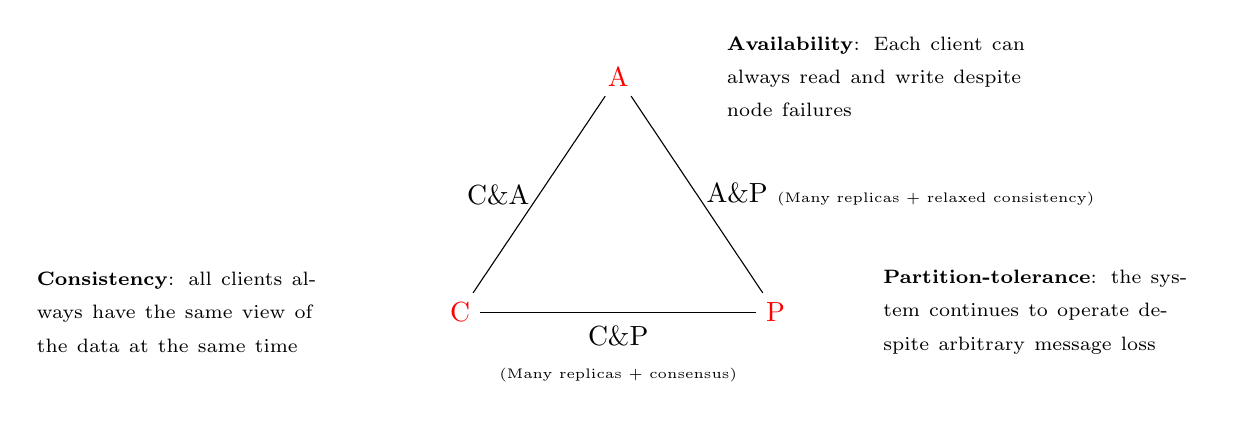
\begin{tikzpicture}
        \node (A) {\textcolor{red}{A}};
        \node (C) [below left= 2.5cm and 1.5cm of A] {\textcolor{red}{C}};
        \node (P) [below right= 2.5cm and 1.5cm of A] {\textcolor{red}{P}};

        \node[right =1cm of A, text width=4cm] {\scriptsize \textbf{Availability}: Each client can always read
        and write despite node failures};

        \node[left =1cm of C, text width=4cm] {\scriptsize \textbf{Consistency}: all clients always have the
        same view of the data at the same time};

        \node[right =1cm of P, text width=4cm] {\scriptsize \textbf{Partition-tolerance}: the
        system continues to operate despite arbitrary message loss};

        \draw (A) edge[-] node[left] {C\&A} (C);
        \draw (A) edge[-] node[right] {A\&P \tiny (Many replicas + relaxed consistency)} (P);
    \draw (C) edge[-] node[below] {\begin{tabular}{c}C\&P\\ \tiny (Many replicas + consensus) \end{tabular}} (P);
    \end{tikzpicture}
\end{center}


\paragraph{Actually}, we have a lot of partition and we have a trade-off
between C and A. \textbf{ACID} (atomicity, consistency, isolation, durability)
become \textbf{BASE} (basically available, soft-state, eventually consistent).


\subsection{Structure}
\begin{figure}[!h]
    \centering
    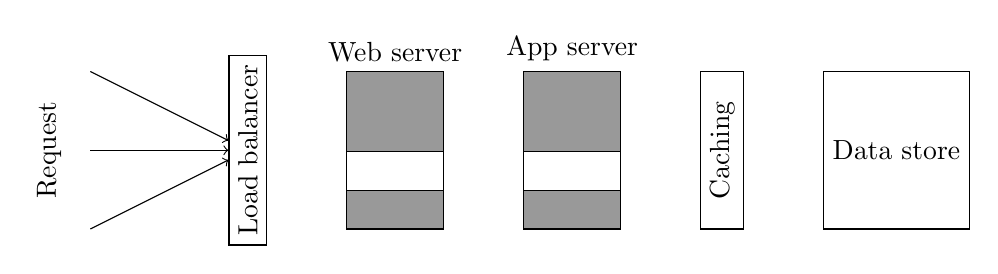
\begin{tikzpicture}

        \node[draw, rectangle, minimum height= 2cm] (L) {\rotatebox{90}{Load balancer}};
        \node[draw, rectangle, fill=black!40, minimum height= 2cm, text width=1cm, right= of L] (W) {};
        \node[draw, rectangle, fill= white, minimum height= 0.5cm, text width=1cm, below=-1cm of W] (W1) {};
        \node[above=0cm of W] (1) {Web server};

        \node[draw, rectangle, fill=black!40, minimum height= 2cm, text width=1cm, right= of W] (A) {};
        \node[draw, rectangle, fill=white, minimum height= 0.5cm, text width=1cm, below=-1cm of A] (A1) {};
        \node[above=0cm of A] (1) {App server};

        \node[draw, rectangle, minimum height= 2cm, right= of A] (C) {\rotatebox{90}{Caching}};
        \node[draw, rectangle, minimum height= 2cm, right= of C] (D) {Data store};

        \draw[->] (-2, 0) -- (L);
        \draw[->] (-2, -1) -- (L);
        \draw[->] (-2, 1) -- (L);

        \node[left=2cm of L] (R) {\rotatebox{90}{Request}};

    \end{tikzpicture}
    \caption{Cloud structure with 
    caching which is central to responsiveness}
\end{figure}

\begin{itemize}
    \item \textbf{Stateless server}: Views a client request as an independent 
        transaction and responds to it


        Easy to scale and more robuste because instance failure does not require
        overheas restoring state

    \item \textbf{Statefull server}: Scaling is challenging because we need to maintains 
        the state.

        \paragraph{Traditionnal approach is replication}:

        \begin{tabular}{m{12cm}m{5cm}}
            \begin{itemize}
                \item Data is written to a \textit{master server} and then
                    replicated to one or more \textit{slave servers}
                    (synchronously or asynchronously)
                \item Read operations can be handled by the slaves
            \end{itemize}
            But in this case, master becomes the write bottleneck and single point of failure.
            &
            \centering
            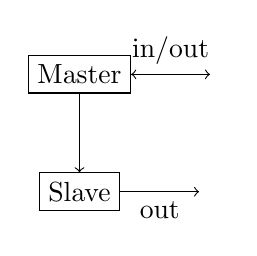
\begin{tikzpicture}
                \node[draw, rectangle] (M) {Master};
                \node[draw, rectangle, below=1cm of M] (S) {Slave};
                \node (I) [right= of M] {};
                \node (O) [right= of S] {};

                \draw[->, double] (I) edge node[above] {in/out} (M);
                \draw[<-, double] (I) edge (M);
                \draw[<-, double] (O) edge node[below] {out}(S);
                \draw[->, double] (M) edge (S);
            \end{tikzpicture}
        \end{tabular}


        \paragraph{Sharding with partitionning}
        The idea is to split data between multiple 
        machines and have a way to make sure that
        the data is available on the right place.
        Typically, define a \textbf{sharding key} and create a \textbf{shard mapping}.

        \begin{tabular}{cm{10cm}}
            This allow to have &
            \begin{itemize}
                \item a really high availability
                \item increase read and write throughput
                \item the possibility 
                    of doing more work in parallel within the application server.
                \item[But] the challenge is to find a good partitionning scheme.
            \end{itemize}
        \end{tabular}

        \textbf{Sharding} is not only for partitioning data 
        within a database, but can also be use to partition data across caching 
        servers (memcached, redis).
\end{itemize}

\paragraph{First-tier parallelism}
Parallelism is vital for fast interactive services, and 
parallel actions must focus on the \textbf{critical path}. This is the
contributor delay for the response delay and do
not care about asynchronous that are shortly.

\begin{center}
    \includegraphics[width=9cm]{img/critical}
\end{center}


Note that update for replicas are typically done in asynchronous way, so we
might not experience much delay on the critical path.

$\rightarrow$ Asynchronous operations decouple systems and 
enable quicker responses at the expense strong 
consistency.
Indeed, this can rise some issues which result in inconsistency:
\begin{itemize}
    \item We don't know in which order replicas applying the update
    \item The leader can crash before replicas change and lose some
        update
\end{itemize}


\section{Cloud storage}

\begin{center}
    \includegraphics[width=12cm]{img/storage}
\end{center}

Many cloud services have a similar structure, 
But the actual storage service is very simple (Read/write 'blocks',
similar to a giant hard disk) and the translation done by the web service.

\paragraph{Ideal store}
\begin{itemize}
    \item Perfect durability – nothing would ever disappear in a crash
    \item 100\% availability – we could always get to the service
    \item Zero latency from anywhere on earth – no delays!
    \item Minimal bandwidth utilization – we only send across the network what we absolutely need
    \item Isolation under concurrent updates – make sure data stays  consistent
\end{itemize}

BUT he “cloud” exists over a physical network (communication take time + limited bandwith)
and The “cloud” has imperfect hardware (failures)

\paragraph{Observation}
\begin{itemize}
    \item Read-­only (or read-­mostly) data is easiest to support
    \item Granularity matters: “Few large-­object” tasks generally 
        tolerate longer latencies than “many small-­object” tasks


        But it’s much more expensive to replicate or to update!

    \item[->] Maybe it makes sense to develop separate solutions for large 
        read-­mostly objects vs. small read-­write objects!
        Different requirements → different technical solutions
\end{itemize}


\subsection{Key-value stores (KVS)}
The key-­value store (KVS) is a simple 
abstraction for managing persistent state where data is 
organized as (key,value) pairs with three basic operation:
\begin{enumerate}
    \item \texttt{PUT(key, value)}
    \item \texttt{value = GET(key)}
    \item \texttt{DEL(key)}
\end{enumerate}

\paragraph{Concurrency control}
Most systems use locks on individual items.



\subsubsection{Amazon dynamo}
\begin{figure}[!h]
    \centering
    \includegraphics[width=5cm]{img/AWSplat}
    \caption{Amazon dynamo. 
        AWS is \textbf{Availability\&Partition-tolerance} and follow 
    \textbf{BASE} philosophy.}
\end{figure}

\begin{tabular}{cm{10cm}}
    Dynamo is :&
    \begin{itemize}
        \item High performance with low latency
        \item High scalable
        \item High available key storage, especially for writes
        \item Partition/fault-tolerant
        \item Eventually consistent (sacrify for high availability)
    \end{itemize}
\end{tabular}
Very low latency writes, reconciliation in reads.

\paragraph{Techniques}
\begin{itemize}
    \item \textbf{Consistent hashing}: dynamically partitions a set of keys
        over a set of storage nodes (hash keys and give 
        a key of m-bits). One key range per virtual node.

        \paragraph{Data partitioning and load balancing}
        A key is assigned to the closest  successor node id 
        (key $k$ is assigned to the first node with $id \geq k$)

        \includegraphics[width=5cm]{img/consistent}

        \begin{center}
            Each node has at most $(1+\epsilon) \frac{K}{N}$ keys with $N$ nodes, $K$ keys
            and $\epsilon=O(log(N))$
            %TODO: why epsilon=0 with virtual nodes?
        \end{center}

        \paragraph{Replication}
        Replication is done on the successors node because if the node fail, it's the successor
        which will take failed node keys.

        \includegraphics[width=5cm]{img/dynamoReplica}

        Replication is may in asynchronous way (eventual consistency), and
        key data versioning technique is done with vector clocks.


        If the replica A in the preference list is down then
        another replica is created on a new node.
        In this case, coordinator will involve D that substitutes
        A until A comes back again. When D gets info A is
        back up it hands back the data to A


    \item \textbf{Vector clocks}: Each write to a key k is associated with a 
        vector clock VC(k) which is an array (map) of integers (one entry VC(k)[i] for each node i).

        This is use for tracking causal dependencies among different versions 
        of the same key (data)

        \includegraphics[width=5cm]{img/vectorClock}

    \item \textbf{Sloppy quorums}: In order to enforce consistency, to response
        to a read or write operation the node must asl to a \textit{quorum}
        which is the minimum number of votes that a distributed transaction has
        to obtain.

        \begin{itemize}
            \item $R$ number of nodes that participate in a get, $W$ number
                of node that participate in a write and $R+W > N$

            \item \textbf{Put}: Generate new $VC$, write locally, send value $VC$
                to N selected nodes from preference list and wait for $W-1$

            \item \textbf{Get}: Send read to $N$ selected nodes from preference list, 
                wait for $R$, select highest versions per $VC$ and return
                all such versions. 

                Writeback merge versions.

            \item[Note]
                \begin{enumerate}
                    \item Note that each node has routing info to all other node
                        to reduce latency (but this is lower scalable)
                        %TODO: slide 99 for 03
                \end{enumerate}
        \end{itemize}

        \textbf{Sloppy} allow availability under a much wider range of 
        partitions (failures) but sacrifice consistency. The
        N selected nodes are the first N healthy 
        nodes.

    \item \textbf{Anti-entropy protocol using hash/merkle tree}:
        Each Dynamo node keeps a Merkle tree for 
        each of its key ranges. Hash trees can be used to verify any kind of data stored.

        \includegraphics[width=5cm]{img/merkle}

        Compares the root of the tree with replicas
        \begin{itemize}
            \item If equal, all keys in a range are equal (replicas in sync)
            \item If not equal 
                Traverse the branches of the tree to pinpoint the children that differ
                The process continues to all leaves
                Synchronize on those keys that differ
        \end{itemize}

    \item \textbf{Gossip-based group membership protocol}: 
        %TODO slides 106 for 03


        Membership info are also eventually 
        consistent — propagated by background 
        gossip protocol.
        \begin{itemize}
            \item Node contacts a random node every 1s
            \item 2 nodes reconcile the membership info and partitioning/placement
                metadata
        \end{itemize}


        \paragraph{Unreliable failure detection (FD)}
        Used to refresh the healthy node info in the extended 
        preference list.

        %TODO 107 for 04

\end{itemize}


\section{MapReduce}

\begin{figure}[!h]
    \centering
    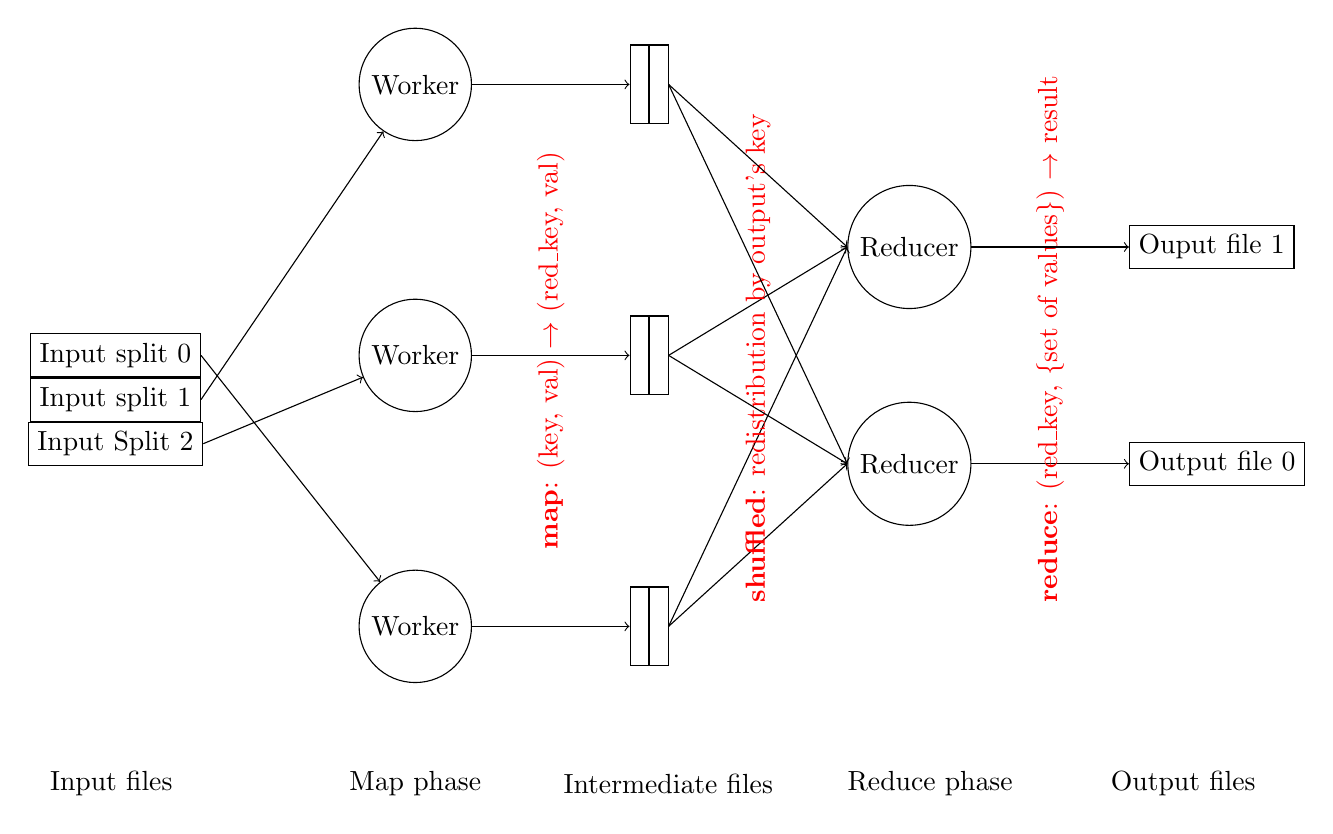
\begin{tikzpicture}[node distance=2cm]
        \node[draw, rectangle] (I0) {Input split 0};
        \node[draw, rectangle, below=0cm of I0] (I1) {Input split 1};
        \node[draw, rectangle, below=0cm of I1] (I2) {Input Split 2};

        \node[draw, circle, right=of I0 ] (W2) {Worker};
        \node[draw, circle, below=of W2 ] (W1) {Worker};
        \node[draw, circle, above=of W2 ] (W3) {Worker};

        \node[draw, minimum height=1cm,rectangle, right=of W1 ] (F1) {};
        \node[draw, minimum height=1cm, rectangle, right=of W2 ] (F2) {};
        \node[draw, minimum height=1cm, rectangle, right=of W3 ] (F3) {};

        \node[draw, rectangle, minimum height=1cm, right=0cm of F1 ] (FF1) {};
        \node[draw, rectangle, minimum height=1cm,right=0cm of F2 ] (FF2) {};
        \node[draw, rectangle, minimum height=1cm, right=0cm of F3 ] (FF3) {};

        \node[draw, circle, above right=1cm and 2.5cm of FF1 ] (R1) {Reducer};
        \node[draw, circle, below right=1cm and 2.5cm of FF3 ] (R2) {Reducer};

        \node[draw, rectangle, right=of R1 ] (O1) {Output file 0};
        \node[draw, rectangle, right=of R2 ] (O2) {Ouput file 1};

        \draw (I0.0) edge[->](W1);
        \draw (I1.0) edge[ ->](W3);
        \draw (I2.0) edge[ ->](W2);

        \draw (W1.0) edge[->] (F1.180);
        \draw (W2.0) edge[->] node 
        {\rotatebox{90}{ \textcolor{red}{\textbf{map}: (key, val) $\rightarrow$ (red\_key, val)}}} (F2.180);
        \draw (W3.0) edge[->] (F3.180);

        \draw (FF1.0) edge[->] (R1.180);
        \draw (FF1.0) edge[->] (R2.180);
        \draw (FF2.0) edge[->] node[below=-2.5cm]
        {\rotatebox{90}{ \textcolor{red}{\textbf{shuffled}: redistribution by output's key}}} (R2.180);
        \draw (FF2.0) edge[->] (R1.180);
        \draw (FF3.0) edge[->] (R1.180);
        \draw (FF3.0) edge[->] (R2.180);

        \draw (R1.0) edge[->] node[above=-2cm]
        {\rotatebox{90}{ \textcolor{red}{\textbf{reduce}: (red\_key, \{set of values\}) $\rightarrow$ result}}} (O1.180); 
        \draw (R2.0) edge[->] (O2.180);

        \node[below=1cm of W1] (2) {Map phase};
        \node[left=of 2] (1) {Input files};
        \node[right=0.8cm of 2] (3){Intermediate files};
        \node[right=0.7cm of 3] (4){Reduce phase};
        \node[right=1cm of 4] (5){Output files};


    \end{tikzpicture}

    \centering
\begin{itemize}
    \item \textbf{File system} distributed across all nodes with replication
    \item \textbf{Driver program} on the master to keeping all node busy
    \item \textbf{Runtime system} which control nodes
\end{itemize}
    \caption{MapReduce where mapper and reducer should be \textbf{stateless}
    }
\end{figure}


A variety  of  different  tasks  can  be  expressed  
as  a  single-­pass  MapReduce program (filtering, aggregation, join on shared
element).
But sorting don't work and algorithms  that  depend  on  shared  global  state  during  
processing  are  difficult  to  implement.


\paragraph{On worker crash} we rely on the  file  system  being  shared  
across  all  the  nodes. 
\begin{itemize}
    \item If the node wrote its  output  and  then  crashed, 
        the  file  system  is  likely  to  have  a  copy  of  the  complete  output.
    \item If the node  crashed  before  finishing  its  output, the master 
        see that  the  job  isn’t  making  progress,  and  restarts  the  
        job  elsewhere  on  the  system
\end{itemize}

\paragraph{Optimization}

\begin{enumerate}
    \item \textit{locality}:  Master tries to do work on nodes that 
        have replicas of the data
    \item \textit{Stragglers}: re-execute slow machines task somewhere else.

    \item \textit{Combiner}: use between mapper and reducer in order to be more efficient.
        Typically, it's job is to pass $(xyz, k)$ instead of $k$ copies of $(xyz, 1)$.
\end{enumerate}

%TODO intersection/join WTF?

\paragraph{Shuffle}

\begin{itemize}
    \item \textbf{Sorting on key}
        Runtime  guarantees  that  reduce  keys  will  be  
        presented  to  reduce in  sorted  order. Shuffle  really
        consists  of two  parts: (1) Partition and (2) Sort.

    \item \textbf{Sorting on value}
        %TODO slide 45 for 04
\end{itemize}


\subsection{Hadoop}

\subsubsection{HDFS}
Hadoop use a distributed file system (HDFS) specialized for particular
types of applications. Files are stored as sets of blocks (64MB) which
are replicated  for  durability  and  availability.

\begin{center}
\includegraphics[width=11cm]{img/hdfs}
\end{center}

\begin{itemize}
    \item Namespace is managed by a single name node and transfert
        is done directly between client and data node
    \item State stored in two files:

        \begin{tabular}{m{7cm}m{9cm}}
        \begin{itemize}
            \item fsimages: snapshot of file system metadata
            \item edits: change since last snapshot
        \end{itemize} &
        \includegraphics[width=9cm]{img/namenode}
    \end{tabular}
\end{itemize}
%TODO slide 65 for 04


\begin{table}[!h]
\begin{tabular}{m{8cm}m{8cm}}
    \textbf{Does well} & \textbf{Does not well} \\
\begin{itemize}
    \item very large read-only or append-only file (Terabytes EASY)
      \item Sequential access parten
      \item High throughput and high capacity
\end{itemize} &
\begin{itemize}
    \item Low-latency access
       \item Multiple writers
       \item Not append-only file
       \item Storing small files
\end{itemize}  \\
& $\rightarrow $ This is well done by Network File System (NFS)
\end{tabular}
\caption{HDFS advantage}
\end{table}
    


\section{Paper}





\end{document}
